\chapterimage{chapter_head_2.pdf} % Chapter heading image
\chapter{Variables, expressions and statements}

\section{Values and types}
\index{value}
\index{type}
\index{string}

A {\bf value} is one of the basic things a program works with,
like a letter or a
number.  The values we have seen so far
are {\tt 1}, {\tt 2}, and
\verb"'Hello, World!'".

These values belong to different {\bf types} also known as {\bf classes} in Python 3. For example,
{\tt 2} is an integer, and \verb"'Hello, World!'" is a {\bf string},
so-called because it contains a ``string'' of letters.
You (and the interpreter) can identify
strings because they are enclosed in quotation marks.

\index{quotation mark}

The print statement also works for integers.

\beforeverb
\begin{pyinterpreter}
>>> print(4)
4
\end{pyinterpreter}
\afterverb
%
If you are not sure what type a value has, the interpreter can tell you.

\beforeverb
\begin{pyinterpreter}
>>> type('Hello, World!')
<class 'str'>
>>> type(17)
<class 'int'>
\end{pyinterpreter}
\afterverb
%
Not surprisingly, strings belong to the type (class) {\tt str} and
integers belong to the type (class) {\tt int}.  Less obviously, numbers
with a decimal point belong to a type called {\tt float},
because these numbers are represented in a
format called {\bf floating-point}.

\index{type}
\index{string type}
\index{type!str}
\index{int type}
\index{type!int}
\index{float type}
\index{type!float}

\beforeverb
\begin{pyinterpreter}
>>> type(3.2)
<class 'float'>
\end{pyinterpreter}
\afterverb
%
What about values like \verb"'17'" and \verb"'3.2'"?
They look like numbers, but they are in quotation marks like
strings.
%
\index{quotation mark}
%
\beforeverb
\begin{pyinterpreter}
>>> type('17')
<class 'str'>
>>> type('3.2')
<class 'str'>
\end{pyinterpreter}
\afterverb
%
They are strings.

When you type a large integer, you might be tempted to use commas
between groups of three digits, as in {\tt 1,000,000}.  This is not a
legal integer in Python, but it is legal:

\beforeverb
\begin{pyinterpreter}
>>> print(1,000,000)
1 0 0
\end{pyinterpreter}
\afterverb
%
Well, that's not what we expected at all!  Python interprets {\tt
  1,000,000} as a comma-separated sequence of integers, which it
prints with spaces between.
%
\index{semantic error}
\index{error!semantic}
\index{error message}
%
This is the first example we have seen of a semantic error: the code
runs without producing an error message, but it doesn't do the
``right'' thing.


\section{Variables}
\index{variable}
\index{assignment statement}
\index{statement!assignment}

One of the most powerful features of a programming language is the
ability to manipulate {\bf variables}.  A variable is a name that
refers to a value.

An {\bf assignment statement} creates new variables and gives
them values:

\beforeverb
\begin{pyinterpreter}
>>> message = 'And now for something completely different'
>>> n = 17
>>> pi = 3.1415926535897931
\end{pyinterpreter}
\afterverb
%
This example makes three assignments.  The first assigns a string
to a new variable named {\tt message};
the second gives the integer {\tt 17} to {\tt n}; the third
assigns the (approximate) value of $\pi$ to {\tt pi}.

\index{state diagram}
\index{diagram!state}

A common way to represent variables on paper is to write the name with
an arrow pointing to the variable's value.  This kind of figure is
called a {\bf state diagram} because it shows what state each of the
variables is in (think of it as the variable's state of mind).
This diagram shows the result of the previous example:

\beforefig
\centerline{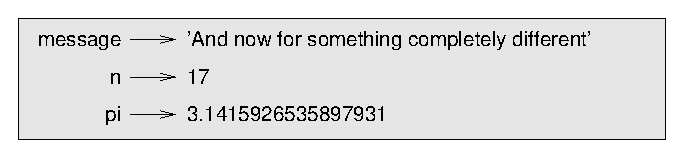
\includegraphics{figs/state2.eps}}
\afterfig

To display the value of a variable, you can use a print statement:

\beforeverb
\begin{pyinterpreter}
>>> print(n)
17
>>> print(pi)
3.14159265359
\end{pyinterpreter}
\afterverb
%
The type of a variable is the type of the value it refers to.

\beforeverb
\begin{pyinterpreter}
>>> type(message)
<class 'str'>
>>> type(n)
<class 'int'>
>>> type(pi)
<class 'float'>
\end{pyinterpreter}
\afterverb
%
\begin{remark}
If you type an integer with a leading zero, you might get
a confusing error:

\beforeverb
\begin{pyinterpreter}
>>> zipcode = 02492
                  ^
SyntaxError: invalid token
\end{pyinterpreter}
\afterverb
\end{remark}




\section{Variable names and keywords}
\index{keyword}

Programmers generally choose names for their variables that
are meaningful---they document what the variable is used for.
Variable names can be arbitrarily long.  They can contain
both letters and numbers, but they have to begin with a letter.
It is legal to use uppercase letters, but it is a good idea
to begin variable names with a lowercase letter (you'll
see why later).
The underscore character (\verb"_") can appear in a name.
It is often used in names with multiple words, such as
\verb"my_name" or \verb"airspeed_of_unladen_swallow".

\index{underscore character}

If you give a variable an illegal name, you get a syntax error:

\beforeverb
\begin{pyinterpreter}
>>> 76trombones = 'big parade'
SyntaxError: invalid syntax
>>> more@ = 1000000
SyntaxError: invalid syntax
>>> class = 'Advanced Theoretical Zymurgy'
SyntaxError: invalid syntax
\end{pyinterpreter}
\afterverb
%
{\tt 76trombones} is illegal because it does not begin with a letter.
{\tt more@} is illegal because it contains an illegal character, {\tt
@}.  But what's wrong with {\tt class}?
It turns out that {\tt class} is one of Python's {\bf keywords}.  The
interpreter uses keywords to recognize the structure of the program,
and they cannot be used as variable names.
Python 3 has 33 keywords has shown in Table~\ref{tab:python_keywords}.
\index{keyword}

\begin{table}[htb]
\begin{center}
\begin{tabular}{p{2cm} p{2cm} p{2cm} p{2cm} p{2cm}}
False & class & finally & is & return\\
None & continue & for & lambda & try\\
True & def & from & nonlocal & while\\
and & del & global & not & with\\
as & elif & if & or & yield\\
assert & else & import & pass & \\
break & except & in & raise & \\
\end{tabular}
\caption{Keywords in Python 3 programming language.}
\label{tab:python_keywords} 
\end{center}
\end{table}
%
You might want to keep this list handy.  If the interpreter complains
about one of your variable names and you don't know why, see if it
is on this list.


\section{Statements}

A statement is a unit of code that the Python interpreter can
execute.  We have seen two kinds of statements: print
and assignment.
%
\index{statement}
\index{interactive mode}
\index{script mode}
%
When you type a statement in interactive mode, the interpreter
executes it and displays the result, if there is one.
%
A script usually contains a sequence of statements.  If there
is more than one statement, the results appear one at a time
as the statements execute.

For example, the script

\beforeverb
\begin{pycode}
print(1)
x = 2
print(x)
\end{pycode}
\afterverb
%
produces the output

\beforeverb
\begin{pyoutput}
1
2
\end{pyoutput}
\afterverb
%
The assignment statement produces no output.


\section{Operators and operands}
\index{operator, arithmetic}
\index{arithmetic operator}
\index{operand}
\index{expression}

{\bf Operators} are special symbols that represent computations like
addition and multiplication.  The values the operator is applied to
are called {\bf operands}.
The operators {\tt +}, {\tt -}, {\tt *}, {\tt /} and {\tt **}
perform addition, subtraction, multiplication, division and
exponentiation, as in the following examples:

\beforeverb
\begin{pyinterpreter}
20+32   hour-1   hour*60+minute   minute/60   5**2   (5+9)*(15-7)
\end{pyinterpreter}
\afterverb
%

%When a variable name appears in the place of an operand, it
%is replaced with its value before the operation is
%performed.

Python 3, as well as other languages have an {\bf integer division} {\tt //}. The integer division operate a {\bf floor division}, that is the operator returns the whole part of the division. The result of the integer division  is an integer. If both operands are integer the value returned is a integer. Otherwise, if at least one of the operand is a float, the value returned is a float.

\beforeverb
\begin{pyinterpreter}
>>> minute = 59
>>> minute // 60
0
>>> minute = 61
>>> minute // 60
1
>>> minute // 60.0
1.0
>>> minute / 60.0
1.0166666666666666
\end{pyinterpreter}
\afterverb
%
\index{Python 3.0}
\index{floor division}
\index{floating-point division}
\index{division!floor}
\index{division!floating-point}
\index{division!integer division}

\section{Expressions}

An {\bf expression} is a combination of values, variables, and operators.
A value all by itself is considered an expression, and so is
a variable, so the following are all legal expressions
(assuming that the variable {\tt x} has been assigned a value):

\index{expression}
\index{evaluate}

\beforeverb
\begin{pycode}
17
x
x + 17
\end{pycode}
\afterverb
%
If you type an expression in interactive mode, the interpreter
{\bf evaluates} it and displays the result:

\beforeverb
\begin{pyinterpreter}
>>> 1 + 1
2
\end{pyinterpreter}
\afterverb
%
But in a script, an expression all by itself doesn't
do anything!  This is a common
source of confusion for beginners.

\begin{exercise}
Type the following statements in the Python interpreter to see
what they do:

\beforeverb
\begin{pyexo}
5
x = 5
x + 1
\end{pyexo}
\afterverb
%
Now put the same statements into a script and run it.  What
is the output?  Modify the script by transforming each
expression into a print statement and then run it again.
\end{exercise}


\section{Order of operations}
\index{order of operations}
\index{rules of precedence}
\index{PEMDAS}

When more than one operator appears in an expression, the order of
evaluation depends on the {\bf rules of precedence}.  For
mathematical operators, Python follows mathematical convention.
The acronym {\bf PEMDAS} is a useful way to
remember the rules:

\index{parentheses!overriding precedence}

\begin{itemize}

\item {\bf P}arentheses have the highest precedence and can be used 
to force an expression to evaluate in the order you want. Since
expressions in parentheses are evaluated first, {\tt 2 * (3-1)} is 4,
and {\tt (1+1)**(5-2)} is 8. You can also use parentheses to make an
expression easier to read, as in {\tt (minute * 100) / 60}, even
if it doesn't change the result.

\item {\bf E}xponentiation has the next highest precedence, so
{\tt 2**1+1} is 3, not 4, and {\tt 3*1**3} is 3, not 27.

\item {\bf M}ultiplication and {\bf D}ivision have the same precedence,
which is higher than {\bf A}ddition and {\bf S}ubtraction, which also
have the same precedence.  So {\tt 2*3-1} is 5, not 4, and
{\tt 6+4/2} is 8, not 5.

\item Operators with the same precedence are evaluated from left to 
right.  So in the expression {\tt degrees/2*pi}, the division
happens first and the result is multiplied by {\tt pi}, therefore the expression is equal to $\frac{\pi}{2}degrees$. To divide by $2 \pi$, you can use parentheses (e.g. {\tt degrees/(2*pi)}) or write {\tt degrees/2/pi}.

\end{itemize}

\begin{table}[htb]
\begin{center}
\begin{tabular}{|p{3cm}|p{7cm}|}
\hline
Operator & Description\\\hline
** & Exponentiation (raise to the power)\\
+, - & Unary plus and minus (method names for the last two are +@ and -@)\\
*, /, \%, //  & Multiply, divide, modulo and floor division\\
+, - & Addition and subtraction\\
%>>, << & Right and left bitwise shift\\
%\& & Bitwise 'AND'\\
%$\hat$, \| & Bitwise exclusive `OR' and regular `OR'\\
<=, <, >, >= & Comparison operators\\
<>, ==, != & Equality operators\\
\verb|is|, \verb|is not| & Identity operators\\
\verb|in|, \verb|not in| & Membership operators\\
\verb|not| & Logical operators\\
\verb|and| & Logical operators\\
\verb|or|  & Logical operators\\
= ,\%=, /=, //=, -=, +=, *=, **= & Assignment operators\\\hline
\end{tabular}
\caption{Operators precedence in Python from highest precedence (top) to lowest (bottom).}
\label{tab:operator_precedence}
\end{center}
\end{table}

\section{String operations}
\index{string!operation}
\index{operator!string}

In general, you cannot perform mathematical operations on strings, even
if the strings look like numbers, so the following are illegal:

\beforeverb
\begin{pyinterpreter}
'2'-'1'    'eggs'/'easy'    'third'*'a charm'
\end{pyinterpreter}
\afterverb
%
The {\tt +} operator works with strings, but it
might not do what you expect: it performs
{\bf concatenation}, which means joining the strings by
linking them end-to-end.  For example:

\index{concatenation}

\beforeverb
\begin{pycode}
first = 'throat'
second = 'warbler'
print(first + second)
\end{pycode}
\afterverb
%
The output of this program is {\tt throatwarbler}.

The {\tt *} operator also works on strings; it performs repetition.
For example, \verb"'Spam'*3" is \verb"'SpamSpamSpam'".  If one of the operands
is a string, the other has to be an integer.
This use of {\tt +} and {\tt *} makes sense by
analogy with addition and multiplication.  Just as {\tt 4*3} is
equivalent to {\tt 4+4+4}, we expect \verb"'Spam'*3" to be the same as
\verb"'Spam'+'Spam'+'Spam'", and it is.  

On the other hand, there is a significant way in which string concatenation 
is different from integer addition. Concatenation is not commutative, which
 means that \verb"'spam'+'sandwich'" is not the same as \verb"'sandwich'+'spam'",
 whereas {\tt 3+4} is the same as {\tt 4+3}.

\index{commutativity}


\section{Comments}
\index{comment}

As programs get bigger and more complicated, they get more difficult
to read.  Formal languages are dense, and it is often difficult to
look at a piece of code and figure out what it is doing, or why.
For this reason, it is a good idea to add notes to your programs to explain
in natural language what the program is doing.  These notes are called
{\bf comments}, and they start with the \verb"#" symbol:

\beforeverb
\begin{pycode}
# compute the percentage of the hour that has elapsed
percentage = (minute * 100) / 60
\end{pycode}
\afterverb
%
In this case, the comment appears on a line by itself.  You can also put
comments at the end of a line:

\beforeverb
\begin{pycode}
percentage = (minute * 100) / 60     # percentage of an hour
\end{pycode}
\afterverb
%
Everything from the {\tt \#} to the end of the line is ignored---it
has no effect on the program.

Comments are most useful when they document non-obvious features of
the code.  It is reasonable to assume that the reader can figure out
{\em what} the code does; it is much more useful to explain {\em why}.

This comment is redundant with the code and useless:

\beforeverb
\begin{pycode}
v = 5     # assign 5 to v
\end{pycode}
\afterverb
%
Such comments are not helping the readability of the code, on the contrary. It is likely that a developer reading your code will stop paying attention to your comments as most of them will be useless. As a consequence, important aspects of your code that have been described in comments will be ignored. On the other hand, the following comment contains useful information that is not in the code:

\beforeverb
\begin{pycode}
v = 5     # velocity in meters/second. 
\end{pycode}
\afterverb
%
Good variable names can reduce the need for comments, but
long names can make complex expressions hard to read, so there is
a tradeoff.

\section{Debugging}
\index{debugging}

At this point the syntax error you are most likely to make is
an illegal variable name, like {\tt class} and {\tt yield}, which
are keywords, or \verb"odd~job" and \verb"GBP£", which contain
illegal characters.

\index{syntax error}
\index{error!syntax}

If you put a space in a variable name, Python thinks it is two
operands without an operator:

\beforeverb
\begin{pyinterpreter}
>>> bad name = 5
SyntaxError: invalid syntax
\end{pyinterpreter}
\afterverb
%
For syntax errors, the error messages don't help much.
The most common messages are {\tt SyntaxError: invalid syntax} and
{\tt SyntaxError: invalid token}, neither of which is very informative.

\index{error message}
\index{use before def}
\index{exception}
\index{runtime error}
\index{error!runtime}

The runtime error you are most likely to make is a \verb|NameError| that is, trying to use a variable before you have assigned a value.  This can happen if you spell a variable name wrong:

\beforeverb
\begin{pyinterpreter}
>>> principal = 327.68
>>> interest = principle * rate
Traceback (most recent call last):
  File "<pyshell#36>", line 1, in <module>
    interest = principle * rate
NameError: name 'principle' is not defined
\end{pyinterpreter}
\afterverb
%
Variables names are case sensitive, so {\tt Principal} is not the
same as {\tt principal}.

\index{case-sensitivity, variable names}
\index{semantic error}
\index{error!semantic}

At this point the most likely cause of a semantic error is
the order of operations.  For example, to evaluate $\frac{1}{2 \pi}$,
you might be tempted to write

\beforeverb
\begin{pyinterpreter}
>>> 1.0 / 2.0 * pi
\end{pyinterpreter}
\afterverb
%
But the division happens first, so you would get $\pi / 2$, which
is not the same thing!  There is no way for Python
to know what you meant to write, so in this case you don't
get an error message; you just get the wrong answer.

\index{order of operations}


\section{Glossary}

\begin{vocabulary}[value:]  One of the basic units of data, like a number or string, 
that a program manipulates.
\index{value}
\end{vocabulary}
	
\begin{vocabulary}[type:] A category of values.  The types we have seen so far
are integers (type {\tt int}), floating-point numbers (type {\tt
float}), and strings (type {\tt str}).
\index{type}
\end{vocabulary}
	
\begin{vocabulary}[integer:] A type that represents whole numbers.
\index{integer}
\end{vocabulary}
	
\begin{vocabulary}[floating-point:] A type that represents numbers with fractional
parts.
\index{floating-point}
\end{vocabulary}
	
\begin{vocabulary}[string:] A type that represents sequences of characters.
\index{string}
\end{vocabulary}
	
\begin{vocabulary}[variable:]  A name that refers to a value.
\index{variable}
\end{vocabulary}
	
\begin{vocabulary}[statement:]  A section of code that represents a command or action.  So
far, the statements we have seen are assignments and print statements.
\index{statement}
\end{vocabulary}
	
\begin{vocabulary}[assignment:]  A statement that assigns a value to a variable.
\index{assignment}
\end{vocabulary}
	
\begin{vocabulary}[state diagram:]  A graphical representation of a set of variables and the
values they refer to.
\index{state diagram}
\end{vocabulary}
	
\begin{vocabulary}[keyword:]  A reserved word that is used by the compiler to parse a
program; you cannot use keywords like {\tt if}, {\tt  def}, and {\tt while} as
variable names.
\index{keyword}
\end{vocabulary}
	
\begin{vocabulary}[operator:]  A special symbol that represents a simple computation like
addition, multiplication, or string concatenation.
\index{operator}
\end{vocabulary}
	
\begin{vocabulary}[operand:]  One of the values on which an operator operates.
\index{operand}

\item[floor division:] The operation that divides two numbers and chops off
the fraction part.
\index{floor division}
\end{vocabulary}
	
\begin{vocabulary}[expression:]  A combination of variables, operators, and values that
represents a single result value.
\index{expression}
\end{vocabulary}
	
\begin{vocabulary}[evaluate:]  To simplify an expression by performing the operations
in order to yield a single value.
\end{vocabulary}
	
\begin{vocabulary}[rules of precedence:]  The set of rules governing the order in which
expressions involving multiple operators and operands are evaluated.
\index{rules of precedence}
\index{precedence}
\end{vocabulary}
	
\begin{vocabulary}[concatenate:]  To join two operands end-to-end.
\index{concatenation}
\end{vocabulary}
	
\begin{vocabulary}[comment:]  Information in a program that is meant for other
programmers (or anyone reading the source code) and has no effect on the
execution of the program.
\index{comment}
\end{vocabulary}
	

\section{Exercises}

\begin{exercise}
Assume that we execute the following assignment statements:

\begin{pyexo}
width = 17
height = 12.0
delimiter = '.'
\end{pyexo}

For each of the following expressions, write the value of the
expression and the type (of the value of the expression).

\begin{enumerate}

\item {\tt width/2}

\item {\tt width/2.0}

\item {\tt height/3}

\item {\tt 1 + 2 * 5}

\item {\tt delimiter * 5}

\end{enumerate}

Use the Python interpreter to check your answers.
\end{exercise}

\begin{exercise}
Practice using the Python interpreter as a calculator: 
\index{calculator}

\begin{enumerate}

\item The volume of a sphere with radius $r$ is $\frac{4}{3} \pi r^3$.
  What is the volume of a sphere with radius 5?  Hint: 392.6 is wrong!

\item Suppose the cover price of a book is \$24.95, but bookstores get a
  40\% discount.  Shipping costs \$3 for the first copy and 75 cents
  for each additional copy.  What is the total wholesale cost for
  60 copies?

\item If I leave my house at 6:52 am and run 1 mile at an easy pace
  (8:15 per mile), then 3 miles at tempo (7:12 per mile) and 1 mile at
  easy pace again, what time do I get home for breakfast?

\index{running pace}

\end{enumerate}
\end{exercise}
